	\chapter{Diseño Arquitectónico}
	
	Tras haber adquirido la información suficiente respecto al conjunto de requisitos objetivos de satisfacción, y del conjunto de tecnologías que deben de integrarse en el proyecto, se muestra a continuación la especificación del diseño arquitectónico.
	
	\vspace{5mm}
	
	El diseño arquitectónico va a describir tanto la estructura arquitectónica del componente de procesos implementado con GO.js, tanto su integración en el producto LUCA, el cual, requiere de un diseño paralelo que implementar.
	
	
	\minitoc
	
	
	Para poder diferenciar estos dos diseños, el componente que implementa GO.JS se nombrará como 'Process Component' y el diseño del producto LUCA que integra el Process Component se llamara 'LUCA Process'.
	
		\section{Process Component}	
		
		Debido a que es un proyecto orientado al entorno gráfico y hará las funciones de widget, el Process-Component ha recibido una arquitectura monocapa, centrándose en ella todos los elementos necesarios para montar una interfaz gráfica.
		
		\vspace{5mm}
		
		Para poder realizarlo, se establecerá una estructura de clases que se comunicará con un framework Javascript llamado GO.JS a través de Vaadin.
			
		\begin{figure}[H]
			\centering
			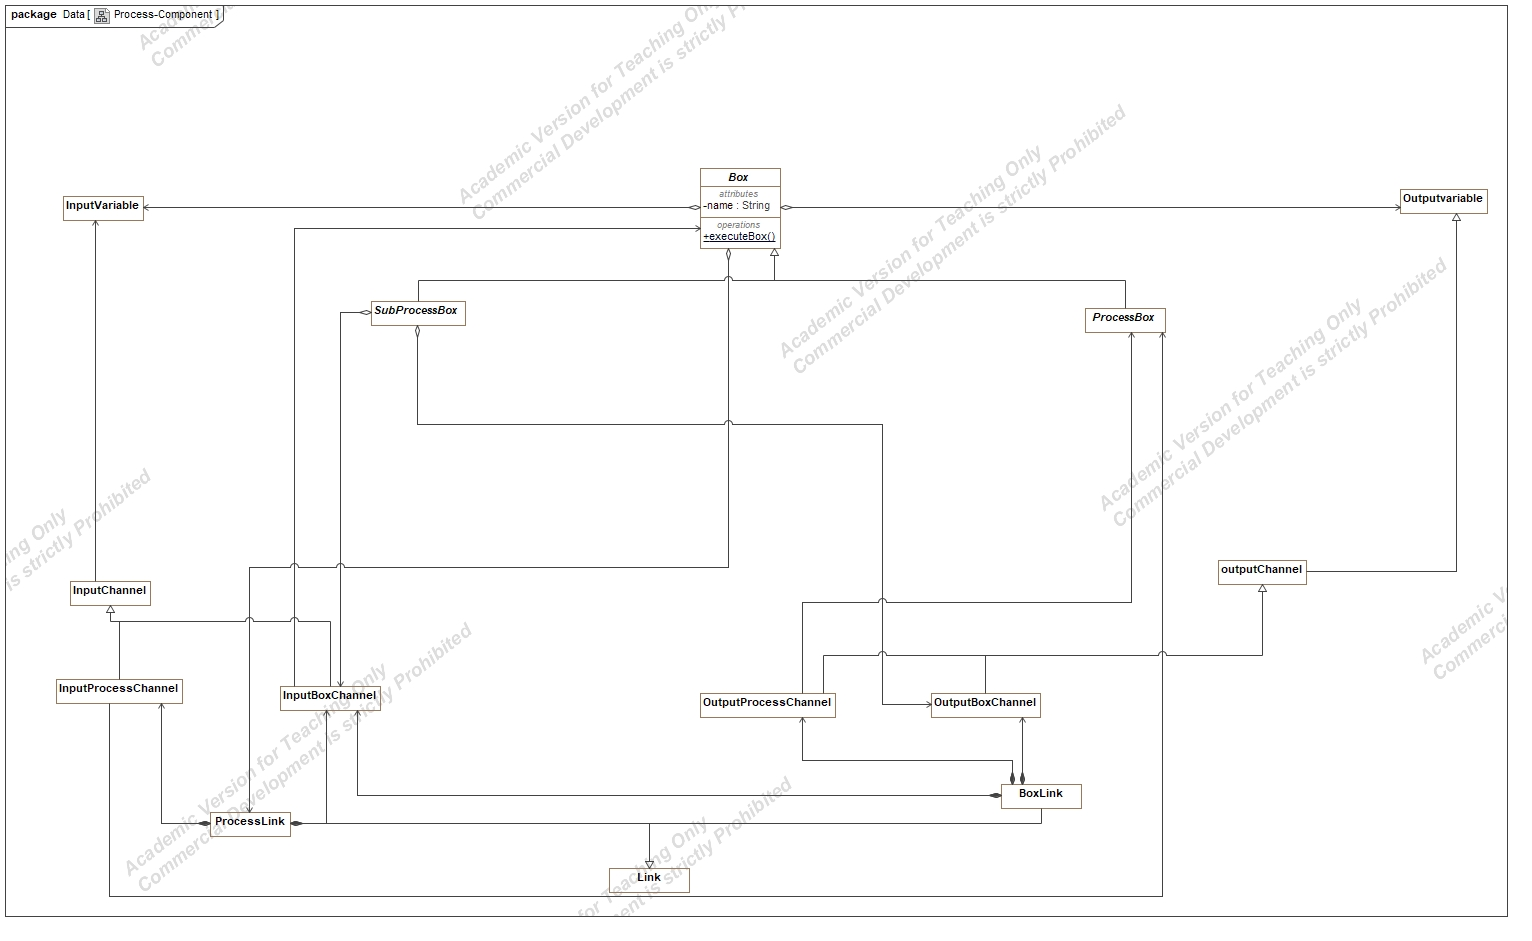
\includegraphics[scale=0.30]{Process-Component.jpg}
			\caption{Diagrama de clases}\label{fig:Process-Component}
		\end{figure}
	
		
		
		\section{Luca Process}
		
		El Luca-Process seguirá un estilo arquitectónico estándar, estará basado en una arquitectura en tres capas convencional\cite{tres-capas}. Esta arquitectura ha sido elegida por varios motivos fundamentales.
		
		\begin{itemize}
			\item Porque es el modelo o esquema que mejor se plantea para este tipo de proyecto que consta de una interfaz gráfica que se comunica con un módulo para realizar transacciones entre ellos. Además, al constar de un apartado de persistencia, es muy beneficioso separar los módulos.
			\item Por capacidad de actuación frente a cambios, de esta forma se pueden cambiar módulos sin afectar al resto.
			\item Por compatibilidad y semejanza con el resto de proyectos y productos desarrollados en la empresa.
			\item Uno primero es porque es un estándar en el conjunto de productos o aplicaciones software.
		\end{itemize} 
		
		\begin{figure}[H]
			\centering
			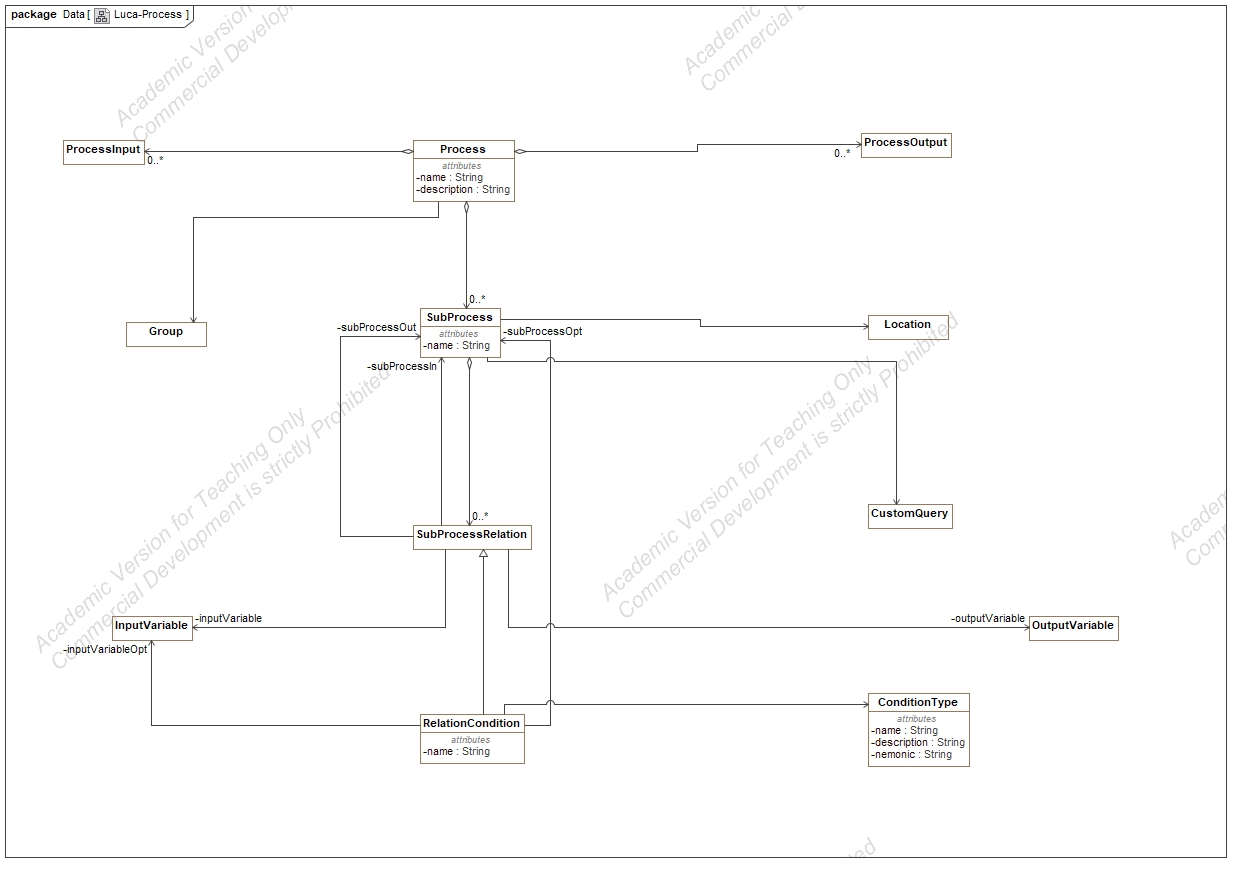
\includegraphics[scale=0.35]{Luca-Process.jpg}
			\caption{Diagrama de clases}\label{fig:Luca-Process}
		\end{figure}
	